\subsection{Mirror Re-coating}

As seen in \F{optics}, each LTCC segment is composed of four optical surfaces: one elliptical mirror, one hyperbolic
mirror, one cylindrical mirror, and the Winston cone. The reflectivity of a random selection of 30 elliptical, cylindrical,
and hyperbolic mirrors from two sectors was measured. All of the mirrors analyzed showed significant degradation
from the original desired reflectivity of 90\% in the visible spectrum, see for example \F{reflectivityBeforeAndAfter}
(top). A refurbishment of the mirrors was crucial to enhance the detector response to the emitted pion Cherenkov
light. Due to the material, assembly, and dimensions of the different types of mirrors, two different techniques were
employed to refurbish the reflective surfaces as discussed below.

\subsubsection{Re-coating of Cylindrical Mirrors}

The cylindrical mirrors range from 6 to 12~in long. Each mirror is made from a single piece of aluminum or plastic. Due
to their small size, they fit in most vacuum chambers used to coat mirrors by evaporation of aluminum with magnesium
fluoride (AlMgF$_2$). After successful testing of AlMgF$_2$ recoating onto the existing substrate, the work of
re-coating the 216 cylindrical mirrors was awarded to ECI~\cite{ECI}. See \F{reflectivityBeforeAndAfter} (bottom)
for typical reflectivity values after re-coating.

\subsubsection{Re-coating of Elliptical and Hyperbolic Mirrors}

The elliptical and hyperbolic mirrors are composed of a Kevlar support structure with a Lexan substrate. It was not
possible to change this hardware from its original design and construction in 1997. The support material, which allowed
for pitch, roll, and yaw alignment of the mirrors, included wood and aluminum pieces that were glued to the support
structure.

\begin{figure}[ht]
\centering
	\includegraphics[width=0.99\columnwidth, height=0.7\columnwidth]{img/mirrorsReflectivityBefore.png}
	\includegraphics[width=0.99\columnwidth, height=0.7\columnwidth]{img/mirrorsReflectivityAfter.png}
	\caption{Top: Reflectivity measurements as a function of wavelength for a sample of 8 mirrors before re-coating,
          each tested at two different places on their surface. The reflectivity was measured using a monochromator
          (Newport model CS260-USB-1-FH-A) with a deuterium light source with a reach between 200~nm and 400~nm.
          The average reflectivity was about 65\% instead of an optimal 90\%. Bottom: Reflectivity measurements as a
          function of wavelength for a sample of 5 mirrors measured after gluing on the Lexan strips (see text for
          details). Note the very high value of reflectivity in the UV region, where most of the Cherenkov light is
          produced. In the visible spectrum, the reflectivity is about 90\%.}
	\label{fig:reflectivityBeforeAndAfter}
\end{figure}

Several companies attempted to re-coat these mirrors but failed due to the outgassing of the various materials.
Furthermore, many of the mirrors are $>$1 m in length, longer than most vacuum chambers. Therefore the AlMgF$_2$
could not be re-deposited directly onto the mirror substrates.

A different approach consisted of coating thin (25~$\mu$m) Lexan strips and gluing the strips onto the mirror
substrate. While promising, this presented the challenge of protecting the coated Lexan strip from shipping and
handling and from the gluing procedure to the mirrors.

A working chain was setup to:

\begin{enumerate}
	\item coat the Lexan strip;
	\item protect the strip with a temporary peel-able film for shipping and handling;
	\item ship to Jefferson Lab;
	\item glue the strip to the mirror substrates;
	\item remove the protective film;
	\item test the reflectivity.
\end{enumerate}

Several companies produced various test samples with various protective material films. The job was eventually awarded
to ECI~\cite{ECI}. The gluing of the strips to the mirror was done at Jefferson Lab. The mirrors were vacuum-mounted
on a supporting structure. Loctite spray contact adhesive glue was applied on the mirror and directed out by a venting
system. The strip was applied to the substrate and after 24 hours of curing time the film was removed. The typical
reflectivity of the refurbished mirrors is shown in \F{reflectivityBeforeAndAfter} (bottom).

\subsubsection{Elliptical Mirror Gaps}

The LTCC elliptical mirrors, especially the longest ones, presented several gaps between the mirrors, some a few
cm long. This was evident also in the data analyses as a loss of efficiency between the mirrors. To make sure that
no light is lost in these gaps, additional 120-$\mu$m thick Lexan extension strips were produced and coated with
AlMgF$_2$. These strips were manufactured by ECI~\cite{ECI}. They were fitted and glued on the left side
elliptical mirrors to cover the gaps, see \F{gapBeforeAndAfter}.

\subsection{Mirror Alignment}
\label{sec:mirrorAlignment}

A new procedure was developed to align the mirrors within the LTCC boxes that takes advantage of their focusing
capabilities. The elliptical mirror focal points (see \F{alignmentSimulation}) are 1. the target (origin of the lab
coordinate system) and 2. a point behind the hyperbolic mirror. The focal points of the hyperbolic mirrors are 1. a
point near the focal point of the elliptical mirrors and 2. a point above the face of the PMTs.

\begin{figure}[hb]
\centering
	\includegraphics[width=0.98\columnwidth, height=0.7\columnwidth]{img/gapBefore.png}
	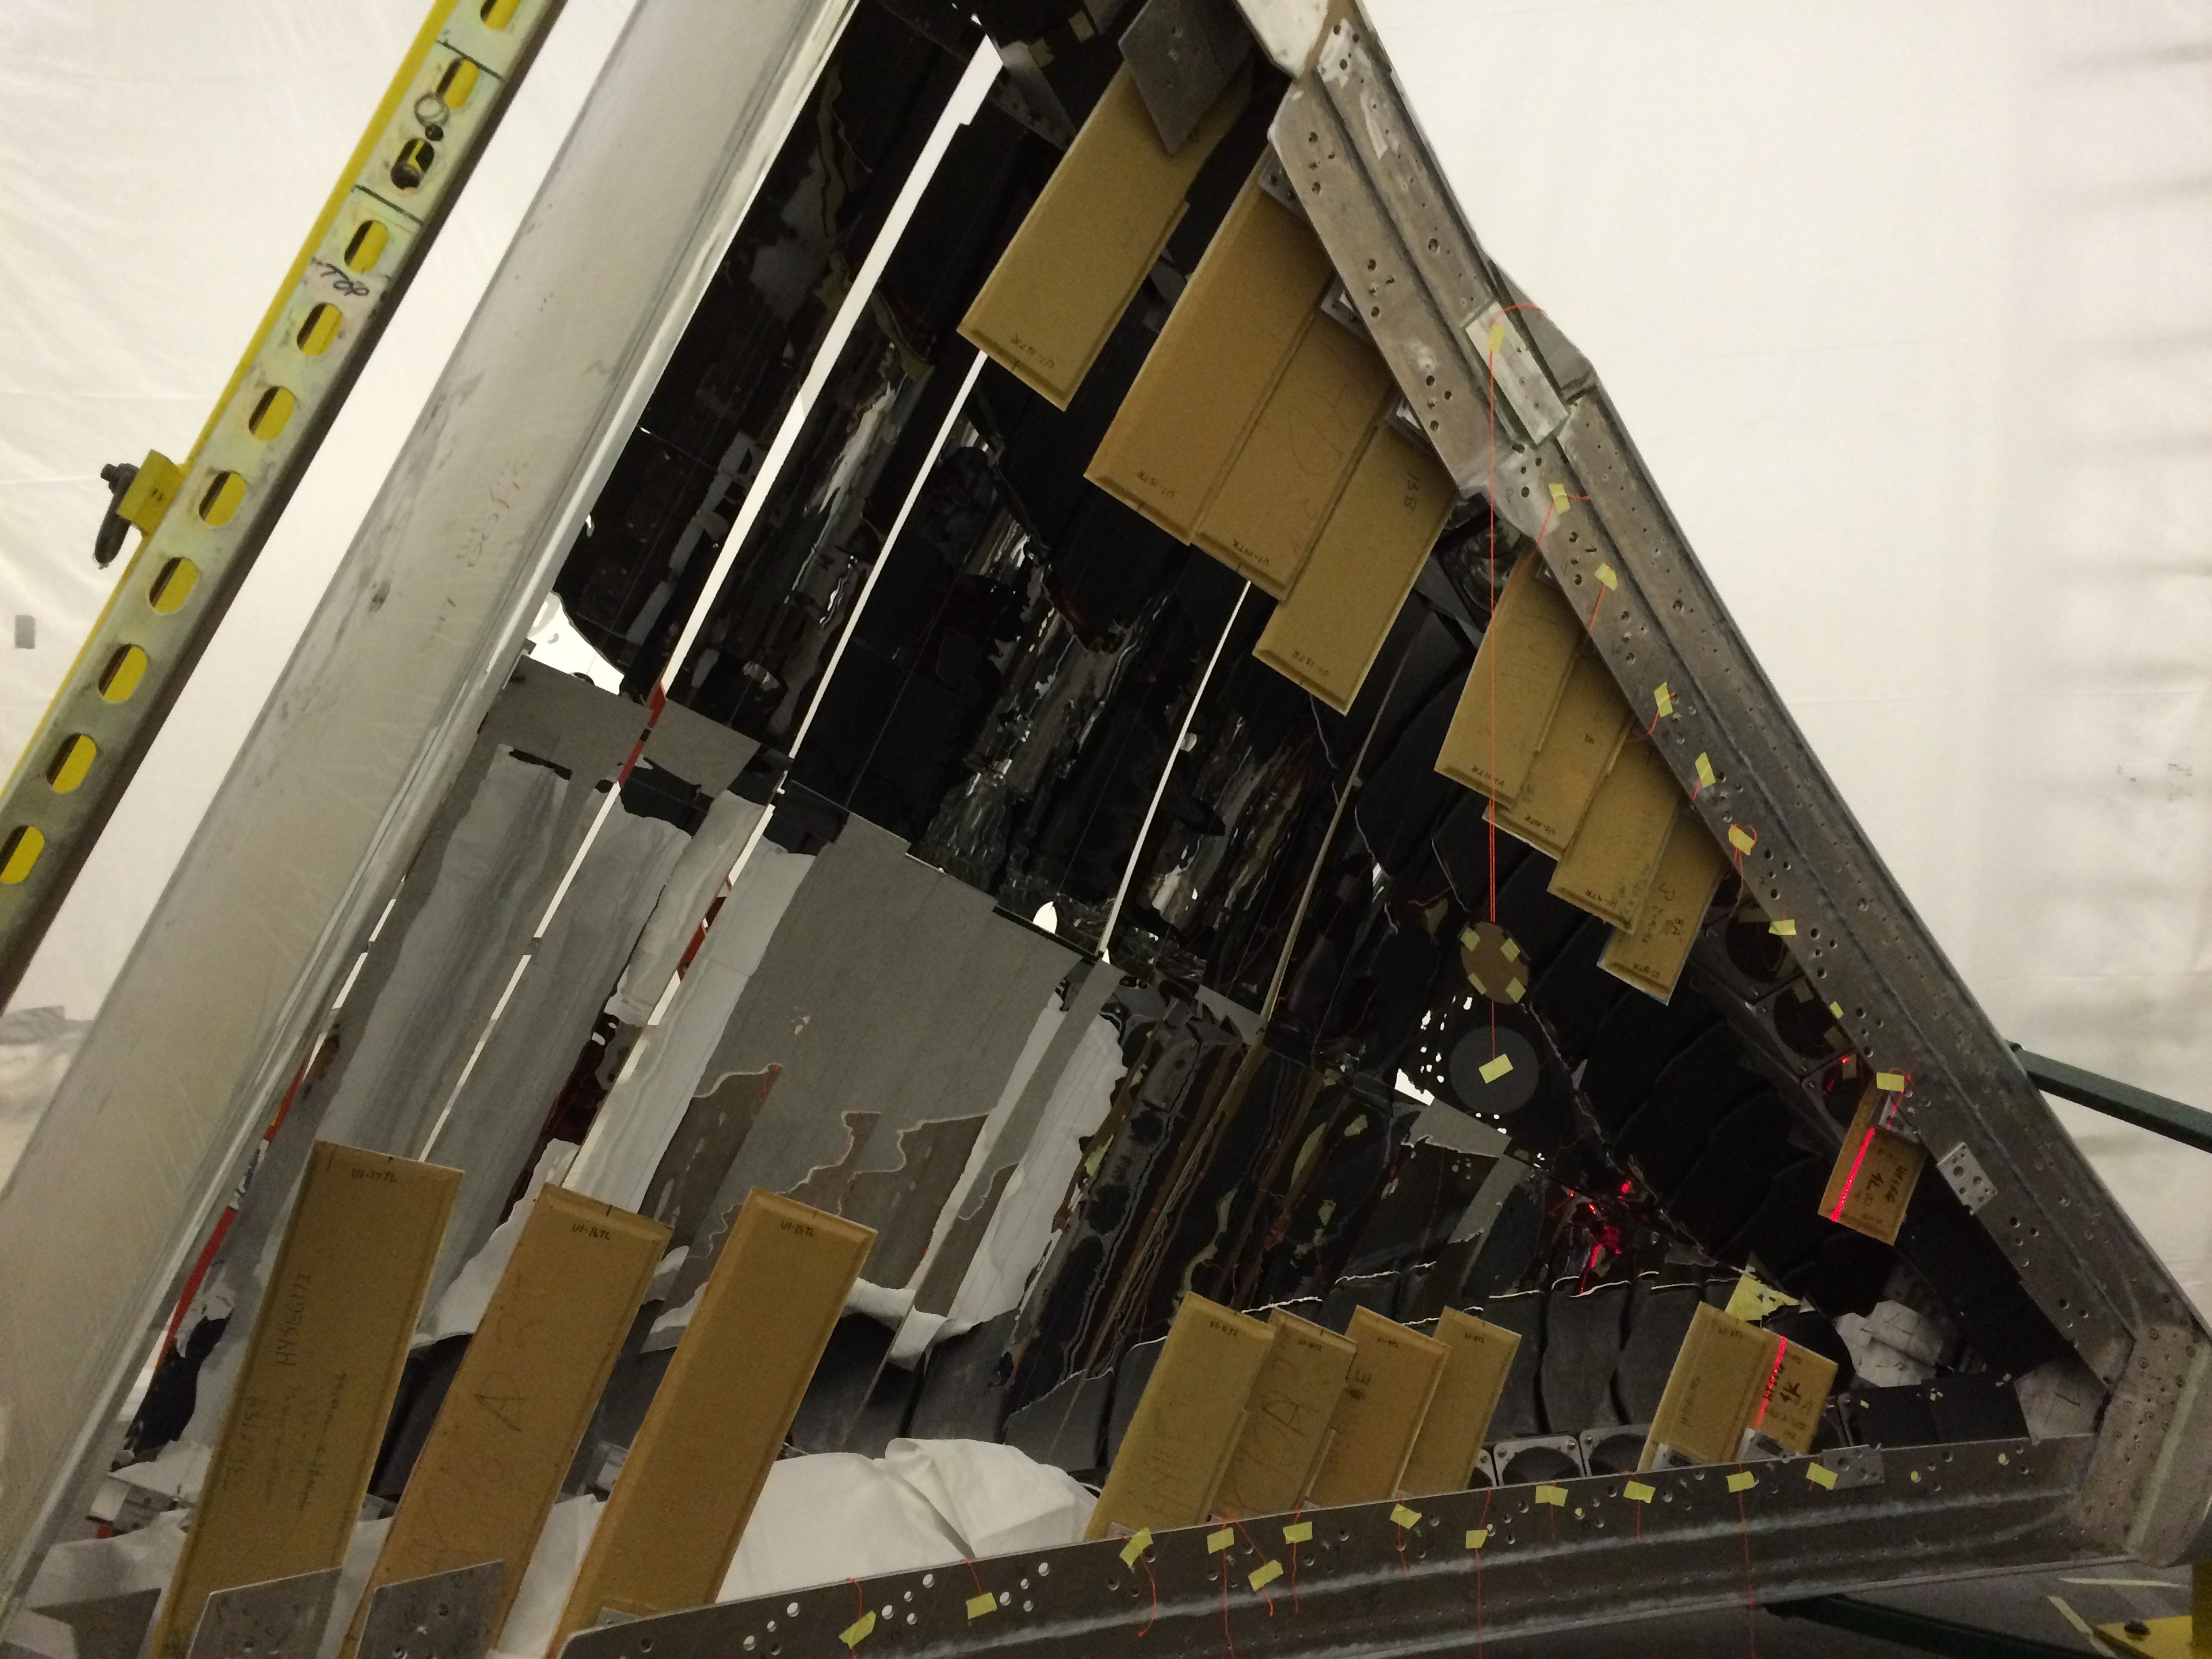
\includegraphics[width=0.98\columnwidth, height=0.7\columnwidth]{img/gapAfter.png}
	\caption{Top: the gaps between mirrors before refurbishing the LTCC. These gaps were also seeing in the data
          as drop of efficiency near the middle of the detector, as the Cherenkov light was not collected. Bottom: all of
          the gaps are covered by the extension strips.}
	\label{fig:gapBeforeAndAfter}
\end{figure}

The geometrical shape of the mirrors has been built into the CLAS12 Geant4 simulation~\cite{sim-nim}. When a laser line
coming from the target is directed at the mirror, it is focused on the hyperbolic focal point, then directed at the PMT,
see \F{alignmentSimulation}. This geometrical focusing was used during the mirror alignment: a 3~mW, 635~nm laser was
placed, relative to the detector, in the center of the CLAS12 coordinate system at the location of the target, and the first
ellipse focal point. The laser was mounted on a structure that allowed the beam direction and line angle to move with respect
to the floor, while keeping the origin of the laser at the coordinate system origin. This position was accurate at the 0.5~mm
level. The laser was spread through two cylindrical lenses into a laser line and shone longitudinally along the center-line of
each elliptical mirror. Both the elliptical and hyperbolic mirrors were then adjusted in pitch, roll, and yaw to minimize the
light spot dimensions and to center it in the middle of the face of the PMT. The PMT entry glasses were protected from
the laser line with custom-fitted cardboard pieces. After alignment, the spot size of the laser was 5~mm.

\subsubsection{Mirrors Overlap and Re-positioning}
\label{sec:possibleInefficiency}

Two issues that could not be fixed in the refurbishment may affect the detector efficiency:

\begin{enumerate}
  \item the mirrors had to be mounted following the original overlaps, see for example \F{gapBeforeAndAfter} top.
    These overlaps were originally implemented to optimize the response to in-bending (toward the beamline) electrons
    and are not optimal for outbending particles.
  \item the relocation of the last four mirror sets (15, 16, 17, and 18) (mentioned in Section~\ref{sec:mirrorRepos})
    may degrade the optics as the affected mirrors do not follow the optimal desired optics configuration with the
    target as the original focal point.
\end{enumerate}

\begin{figure}
\centering
	\includegraphics[width=0.99\columnwidth,  height=0.75\columnwidth]{img/mirrorAlignmentSimulationZoomed.png}
	\caption{The simulation of a laser line (white tracks are photons) originating from the target (first ellipse focal
          point) and directed at the elliptical mirrors. The photons are reflected to the second ellipse focal point. The
          hyperbole first focal point is near the ellipse focal point so the hyperbolic mirror reflects the incoming photons
          to the hyperbole second focal point, located above the face of the PMTs. This picture illustrates the procedure
          used for the alignment: the mirror positions were adjusted until the laser line originating from the target was
          focused on the face of the PMT.}
	\label{fig:alignmentSimulation}
\end{figure}

